
	\begin{enumerate}
		\item Дата собрания: 5.11.14
		\item Цель:
		\begin{itemize}
			\item Полностью собрать подъемник и испытать его
			\item Написать программу для управления им
		\end{itemize}			
		\item Реализация:
		\begin{itemize}
			\item Подъемник был собран, под стяжки пришлось расширить уже просверленные отверстия
			\item Механизм передвижения подъемника был переделан на более простой.
		\end{itemize}
		\item Результаты:
		\begin{itemize}
			\item Шестеренки при подъеме конструкции соскальзывали из-за слишком большого усилия, оси слишком сильно выгибались по той же причине.
		\end{itemize}
		\item Идеи и планы:
		\begin{itemize}
			\item Поставить меньшее передаточное отношение
			\item Установить более прочные оси
			\item Скрепить прочной жёсткой балкой оси, на которых располагаются шестерёнки
		\end{itemize}
		\begin{figure} [h]
			\centering
			\begin{minipage}{0.3\linewidth}
				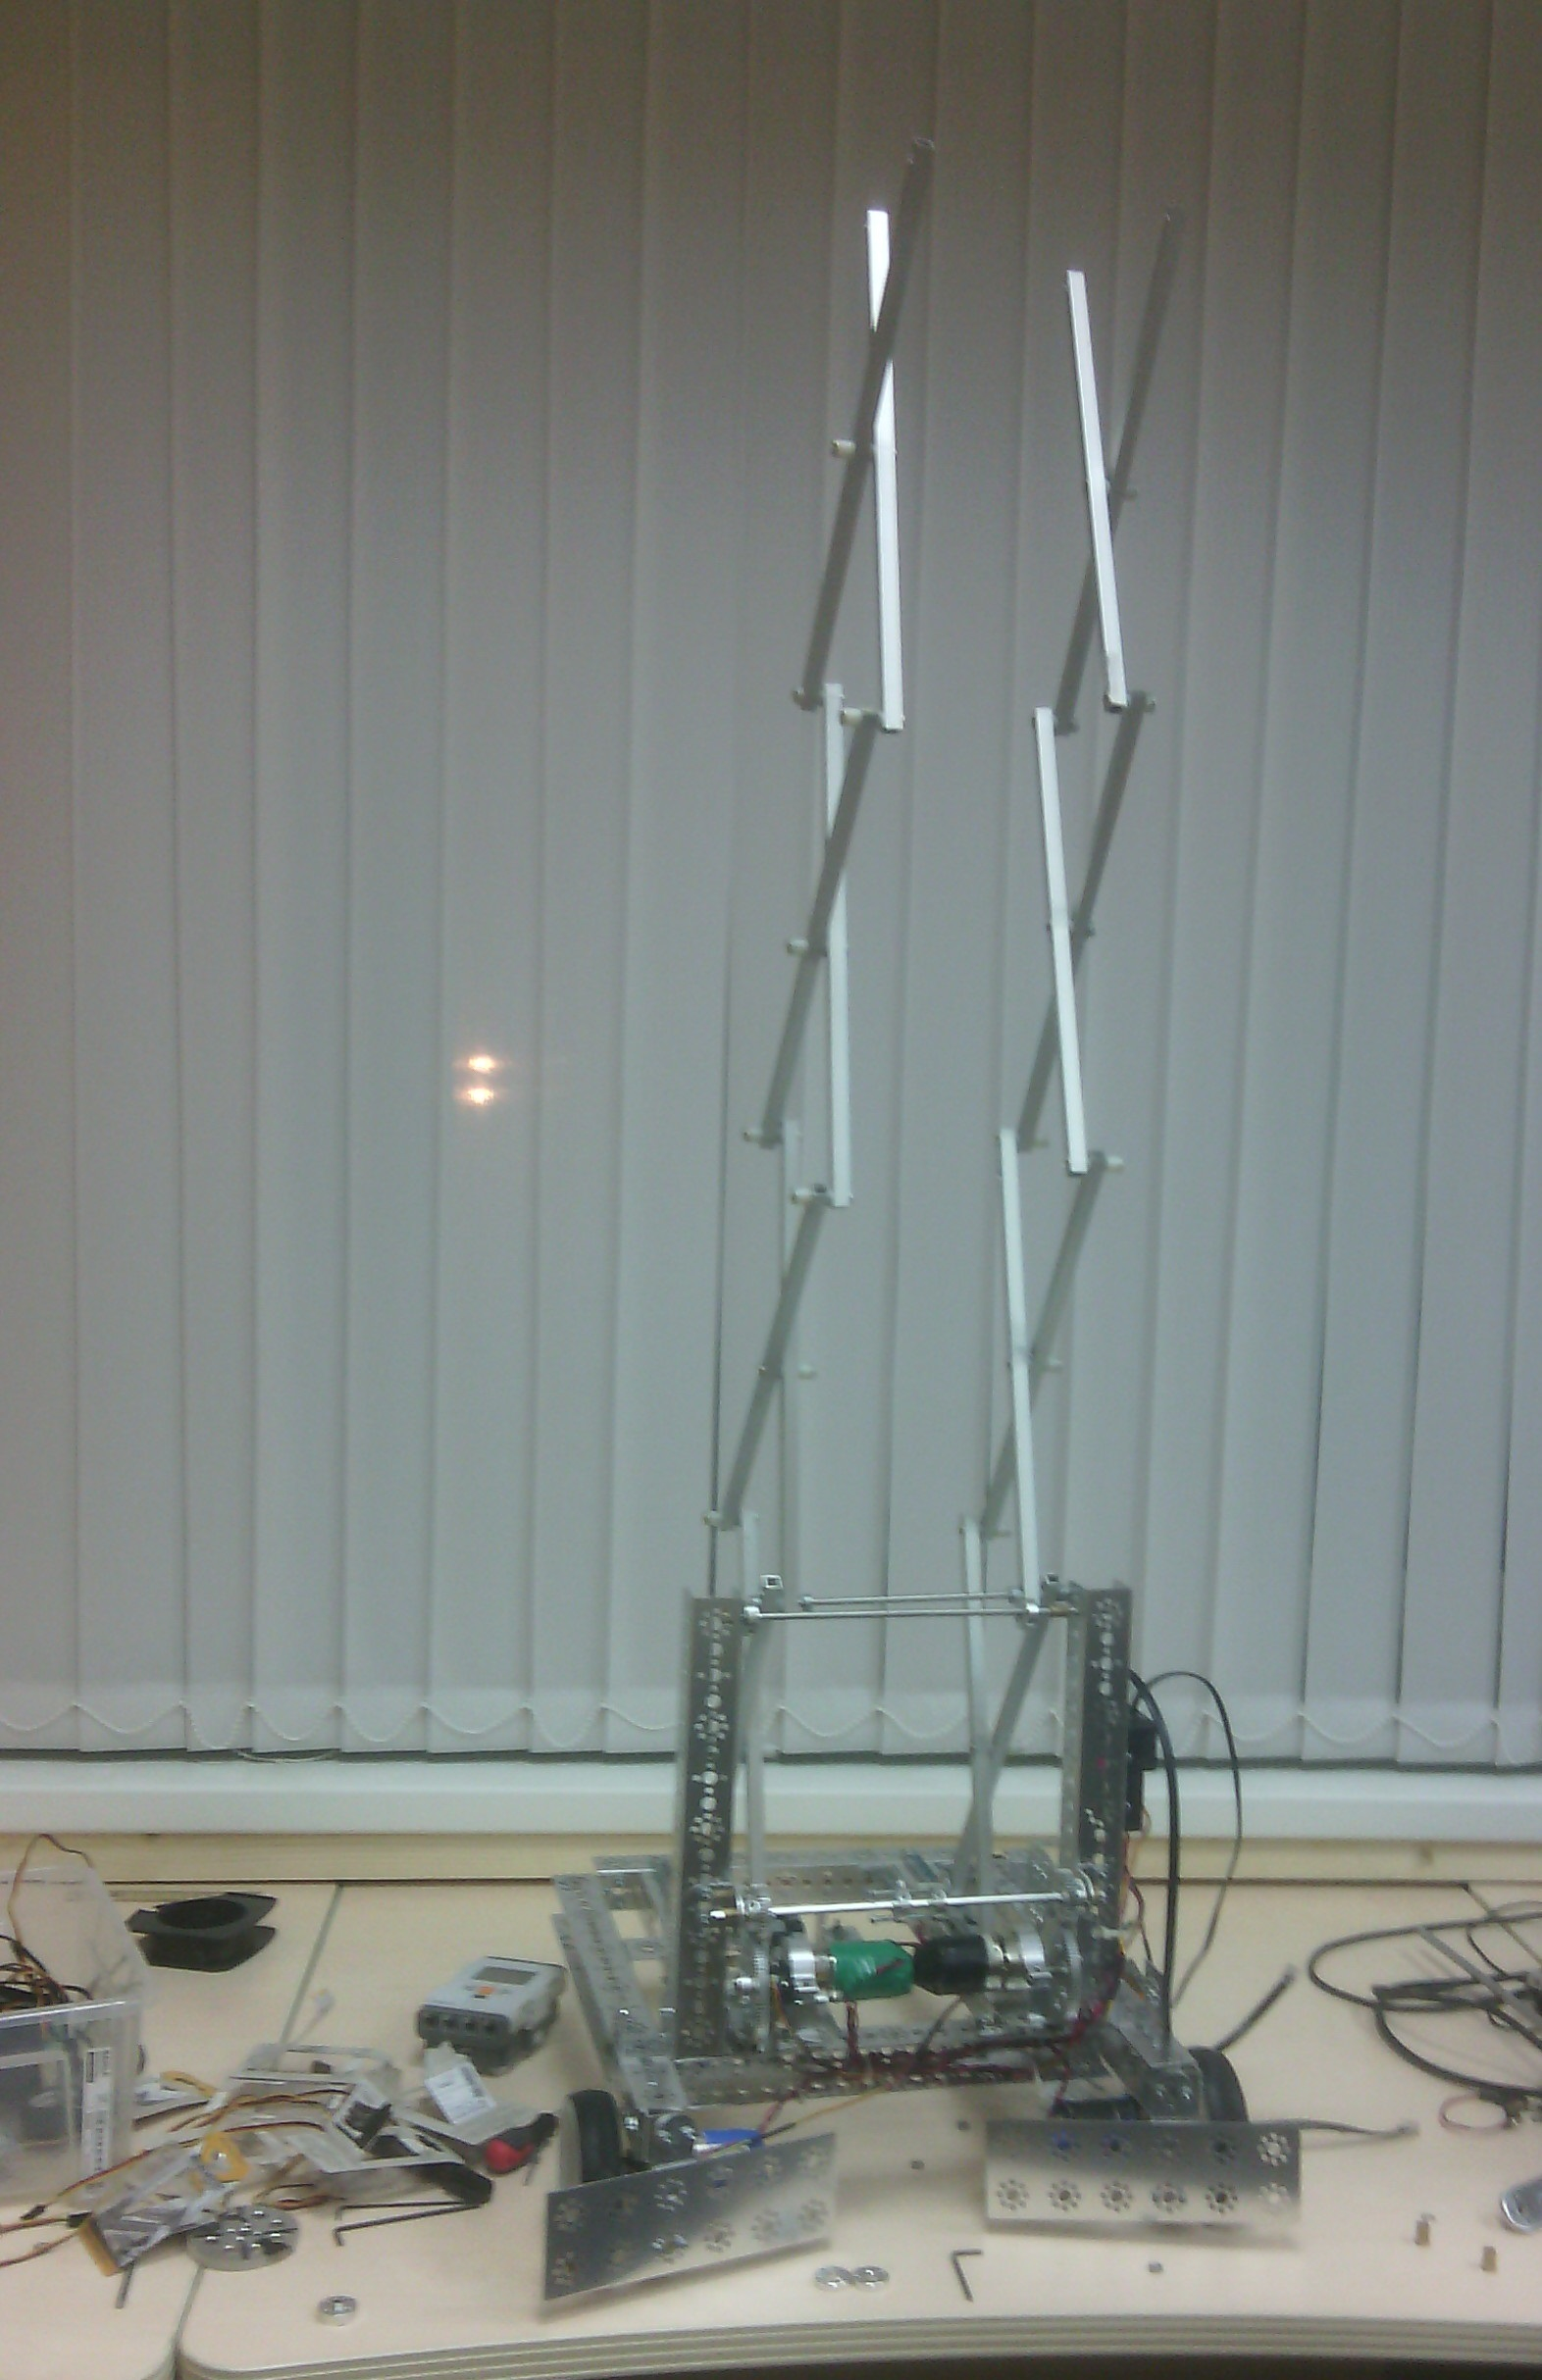
\includegraphics[width=45mm,height=40mm]{Days/5.11.14/10_1_robot}\\ Рисунок 14
			\end{minipage}
			\begin{minipage}{0.3\linewidth}
				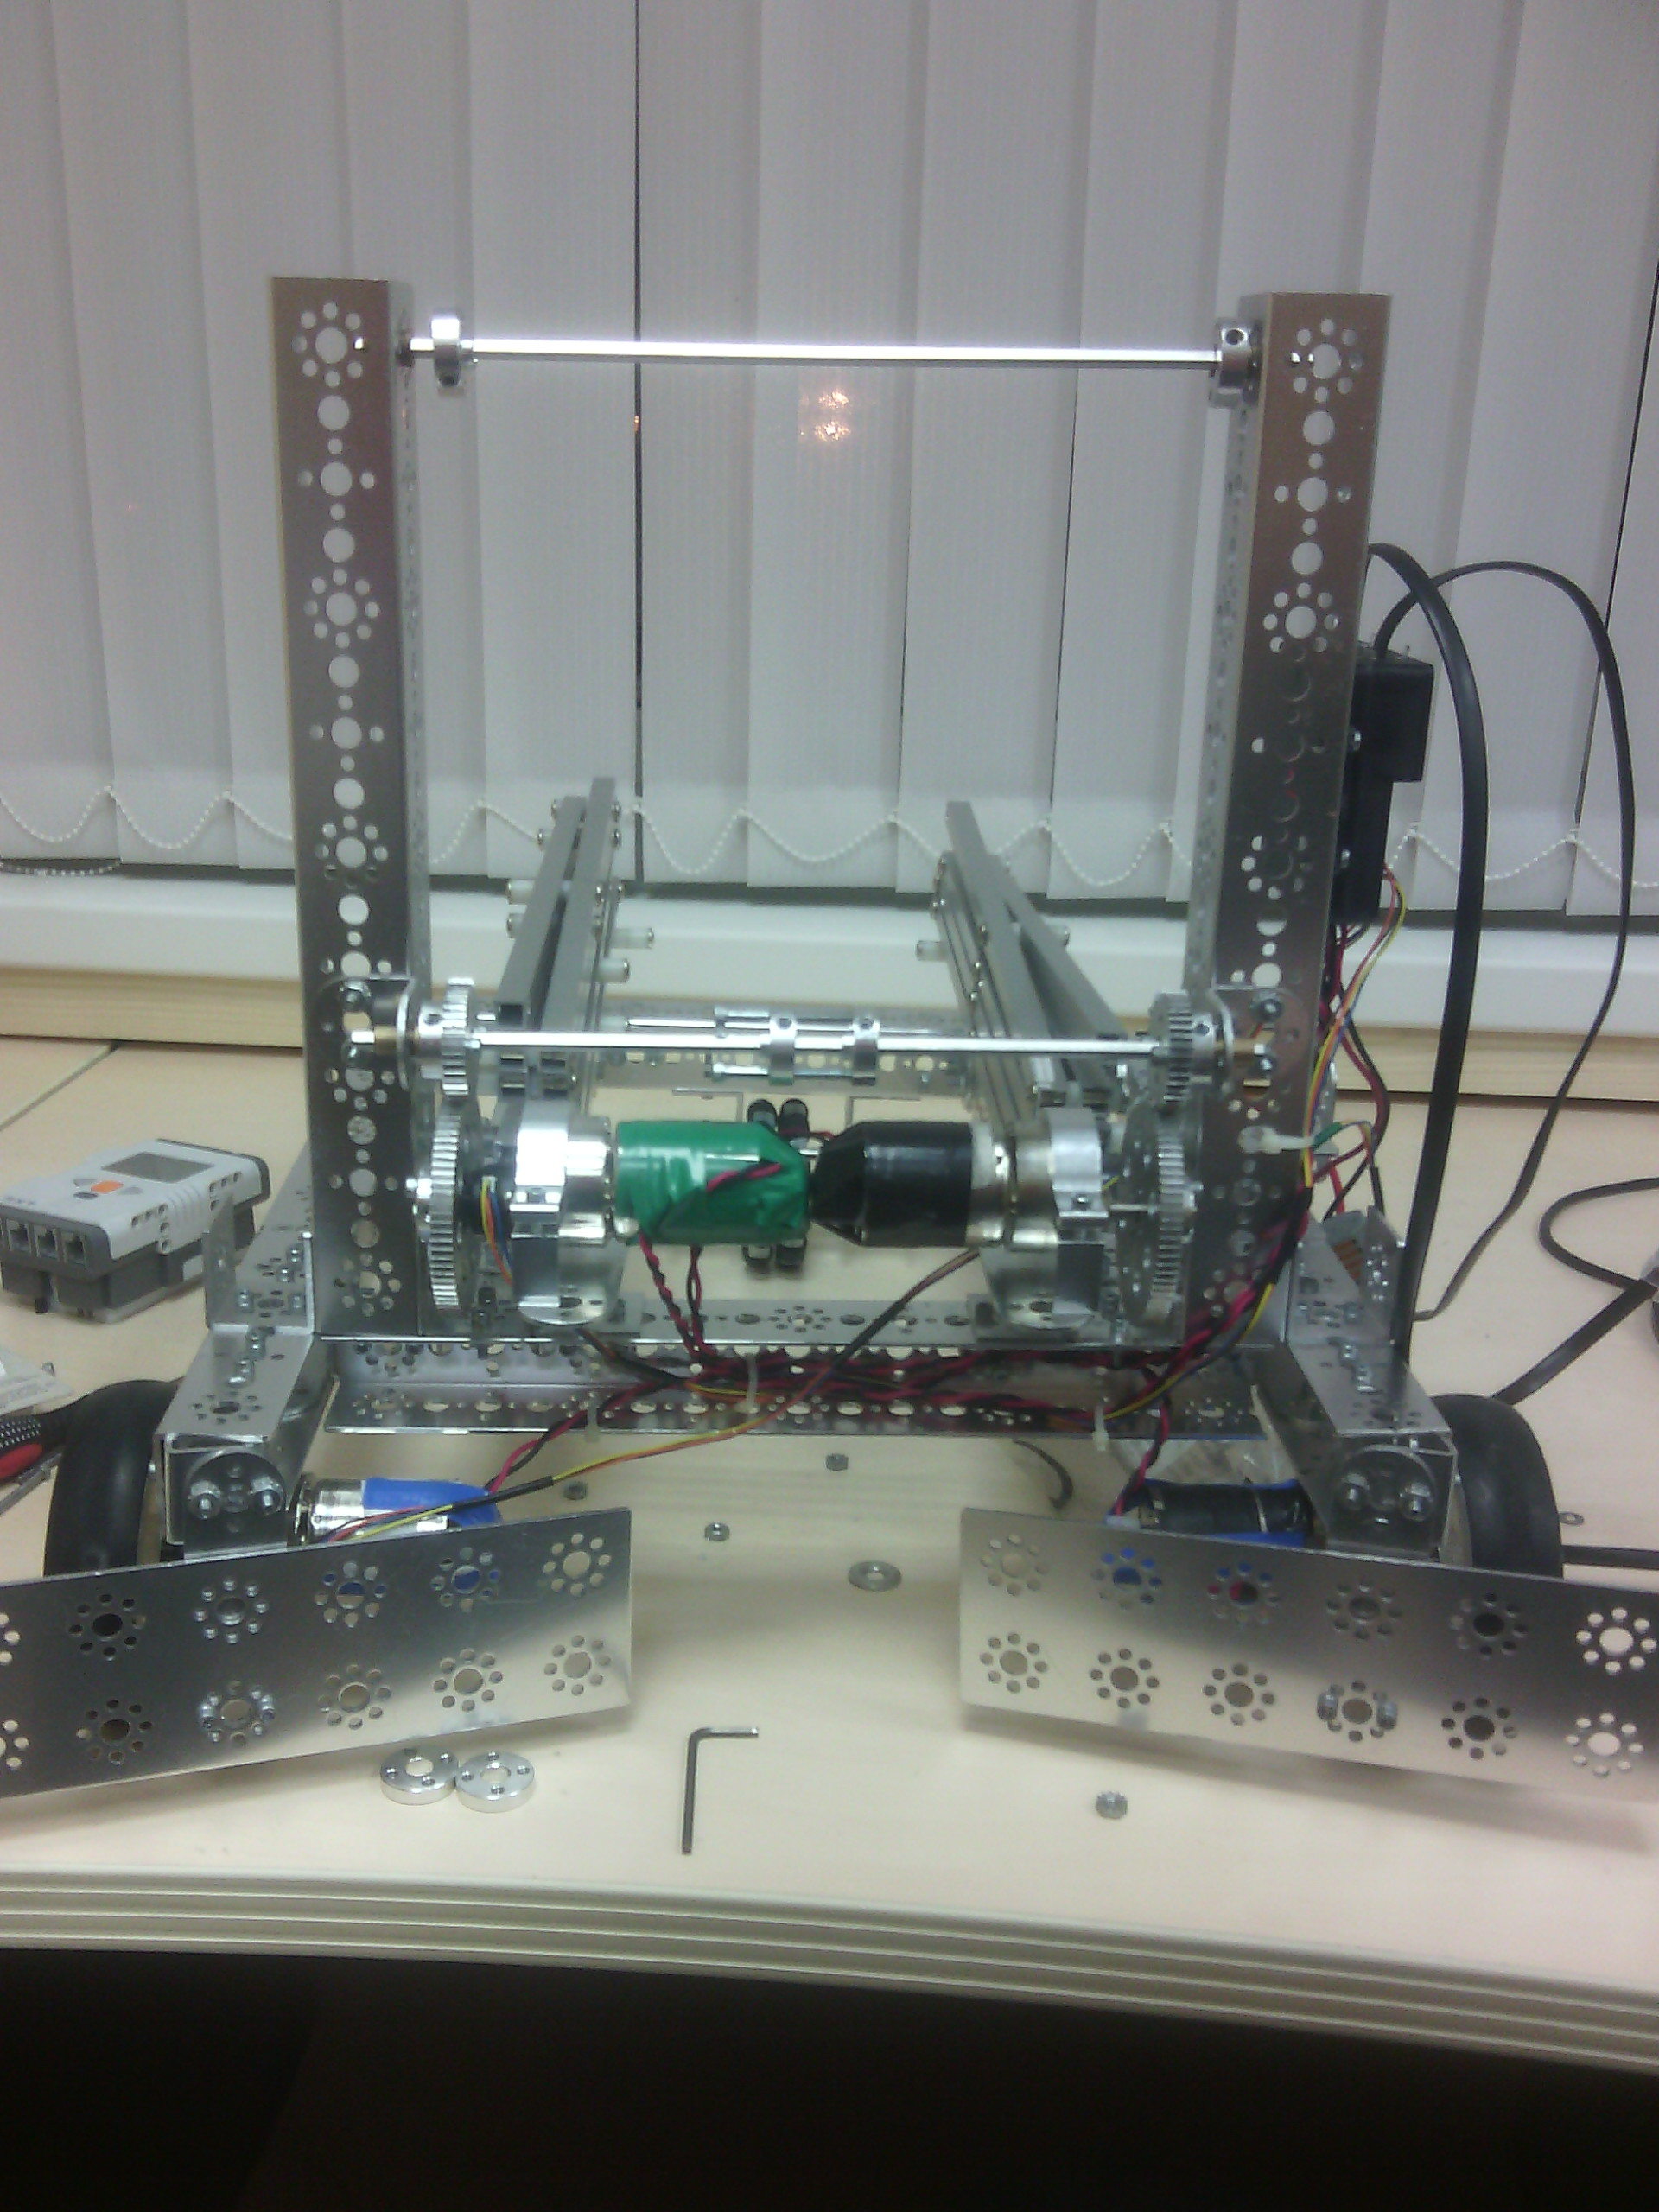
\includegraphics[width=45mm,height=40mm]{Days/5.11.14/10_3_robot}\\ Рисунок 15
			\end{minipage}
		\end{figure}
	\end{enumerate}
\fillpage